\chapter{Implementation}
\label{ch:implementation}


In this chapter, a concrete implementation of the proposed approach is discussed. 
Details about significant modules and practical use cases of RDF-Doctor  are presented in the following.  
 
\section {Modules} 

The implementation of RDF-Doctor is composed of several modules.
{Figure~\ref{Fig:UML}} illustrates a UML diagram of the three most important modules: Orchestration, Detection, and Correction. 
The following text discusses these modules as well as the so-called Core module.
	\begin{figure}[ht]
	\begin{center}
		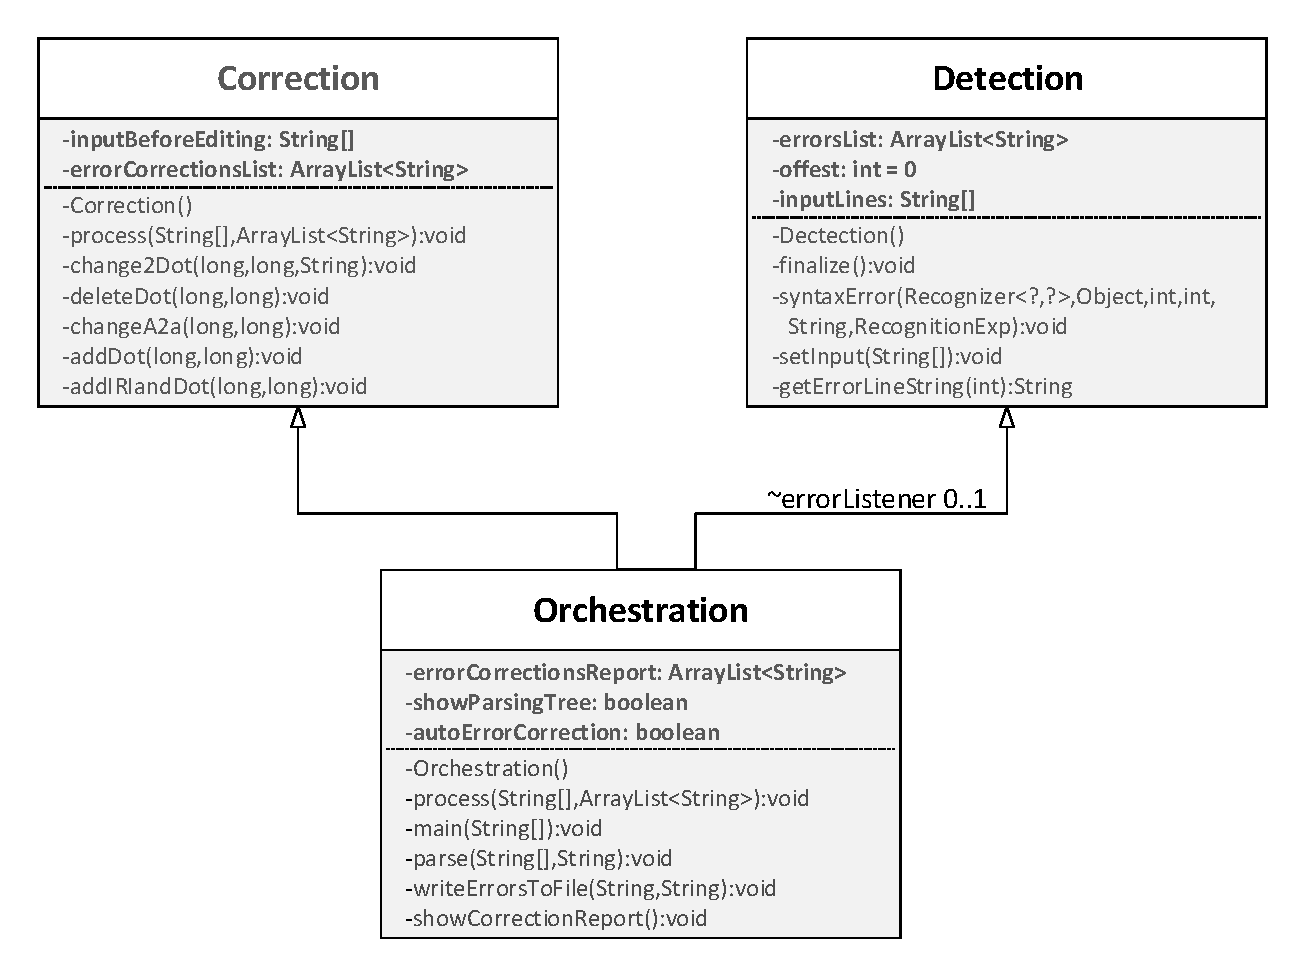
\includegraphics[scale=0.65,angle=0]{images/methods.pdf}
		\setlength{\abovecaptionskip}{0pt} 
				\setlength\belowcaptionskip{-5mm}
		\caption{\textbf{Modules of RDF-Doctor.} 
		Three main modules of RDF-Doctor. 
		Orchestration module parses RDF input and encountered errors are collected by \emph{errorListener}.
		The \emph{Detection} method handles errors collected in errorlistener and releases the appropriate error messages.
		Finally, the \emph{Correction} method perform recovery actions to certain errors.}
		\label{Fig:UML}
	\end{center}
\end{figure}


\begin{enumerate}[]
 \item \textbf {Core}: is automatically generated by ANTLR based on the predefined grammar, which is listed in Appendix \ref{ch:appendix}. 
 It encloses parsing classes, such as Parser, Lexer, Error Listener, Parse Tree Creator, etc. This module is not shown in Figure \ref{Fig:UML} since it is automatically generated and the focus in this chapter is to show our actual developed modules. 
\item \textbf{Detection}: an error detection module listens to the generated error messages, released by the parser. 
Commonly, during parsing procedure, if the parser detects syntax errors, it sends a notification to the error listener API. 
This module enriches the list of errors that are collected by the error listener API with valuable information about the errors, such as  expressive messages to describe the actual error,  error locations, identified by line and column numbers, and usually  actual text lines  of the input where the parser has discovered such a particular error.

\item \textbf {Correction}: a module that corrects the detected syntax errors whenever a well-known error resolving solution is available. 
The error message plays an important role to identify whether such an error can be corrected or not. 
A global list stores all detected syntax errors, including their messages and location in the input file. 
If any of the detected error messages matches any of the predefined messages, then such error can be recovered.

\item \textbf{Orchestration}: %\todo{Maybe rename this module, instead of Main to "Orchestration", dont forget also in the Diagram} 
is the executive module which combines input, output, and processing components. 
It receives the input text, and if it of a large-volume (for example, more than 1 million lines), it is sliced into  chunks. In addition, each chunk is handled separately, in regard to parsing, error detection, as well as error correction.

\end{enumerate} 


\section{Use Cases in Practice}
In this section, some of use cases tackled in this study to detect syntax errors and correct some of the detected syntax errors are elaborated. 
First, we start with a Turtle example which has no syntax errors, then some syntax errors are introduced to show the process of handling them. 


\begin{lstlisting}[label=lst:turtleExample, numbers=left, caption={RDF example in Turtle serialization format}]
<@\textcolor{blue}{@prefix}@>  <@\textcolor{red}{rdf}@>: <@\textcolor{orange}{<http://www.w3.org/1999/02/22-rdf-syntax-ns\#>}@> .
<@\textcolor{blue}{@prefix}@>  <@\textcolor{red}{rdfs}@>:  <@\textcolor{orange}{<http://www.w3.org/2000/01/rdf-schema\#>}@> .
<@\textcolor{blue}{@prefix}@>  <@\textcolor{red}{ex}@>:  <@\textcolor{orange}{<http://example.org/>}@> .
<@\textcolor{blue}{@prefix}@>  <@\textcolor{red}{zoo}@>:   <@\textcolor{orange}{<http://example.org/zoo/> }@> .
<@\textcolor{red}{ex}@>:dog1  <@\textcolor{red}{rdf}@>:type  <@\textcolor{red}{ex}@>:animal .
<@\textcolor{red}{ex}@>:cat1  <@\textcolor{red}{rdf}@>:type  <@\textcolor{red}{ex}@>:cat ;
         <@\textcolor{red}{rdfs}@>:label   <@\textcolor{green}{"Lusi"@en}@> .
<@\textcolor{red}{ex}@>:cat  <@\textcolor{red}{rdfs}@>:subClassOf  <@\textcolor{red}{ex}@>:animal .
<@\textcolor{red}{zoo}@>:host  <@\textcolor{red}{rdfs}@>:range  <@\textcolor{red}{ex}@>:animal .
<@\textcolor{red}{ex}@>:zoo1  <@\textcolor{red}{zoo}@>:host  <@\textcolor{red}{ex}@>:cat2 .
\end{lstlisting}

Listing \ref{lst:turtleExample} shows a Turtle example without syntax errors. 
The first four lines are directives or prefixes declaration whereas in the rest of lines several triples are listed.  
For that reason, our grammar in Appendix~\ref{ch:appendix} is initialized with the topmost node \textbf{start} which describes the coming rules by zero or more  \textbf{statement}(s). 
In addition, each \textbf{statement} is either a directive or a triple as it is represented in Listing~\ref{lst:startingRules}.

\begin{lstlisting}[label=lst:startingRules,
caption={Starting rules in the grammar file}] 
start
: statement*  EOF
;
statement
: directive
| triples '.'
;
\end{lstlisting}

To shed light on the generated parse tree for Listing~\ref{lst:turtleExample}, Figure \ref{Fig:implementationParseTreeLeft}
and Figure \ref{Fig:implementationParseTreeRight}
were depicted. The former shows how does RDF-Doctor parse the first two lines of  Listing~\ref{lst:turtleExample}, it can be seen that those lines come under \emph{prefixID} since they match Prefix patterns. Meanwile, the latter demonstrates a view of the parse tree for the first 3 lines after prefixes: lines 5, 6, and 7, as well as \emph{EndOfFile} (EOF) sequence. Line 5 matches \emph{triple} with only one subject \emph{ex:dog1}, but lines 6, and 7 match \emph{triple} with multiple predicates and objects and share the same subject \emph{ex:cat1}, same is applied on the parse tree.  





\begin{figure}
		\centering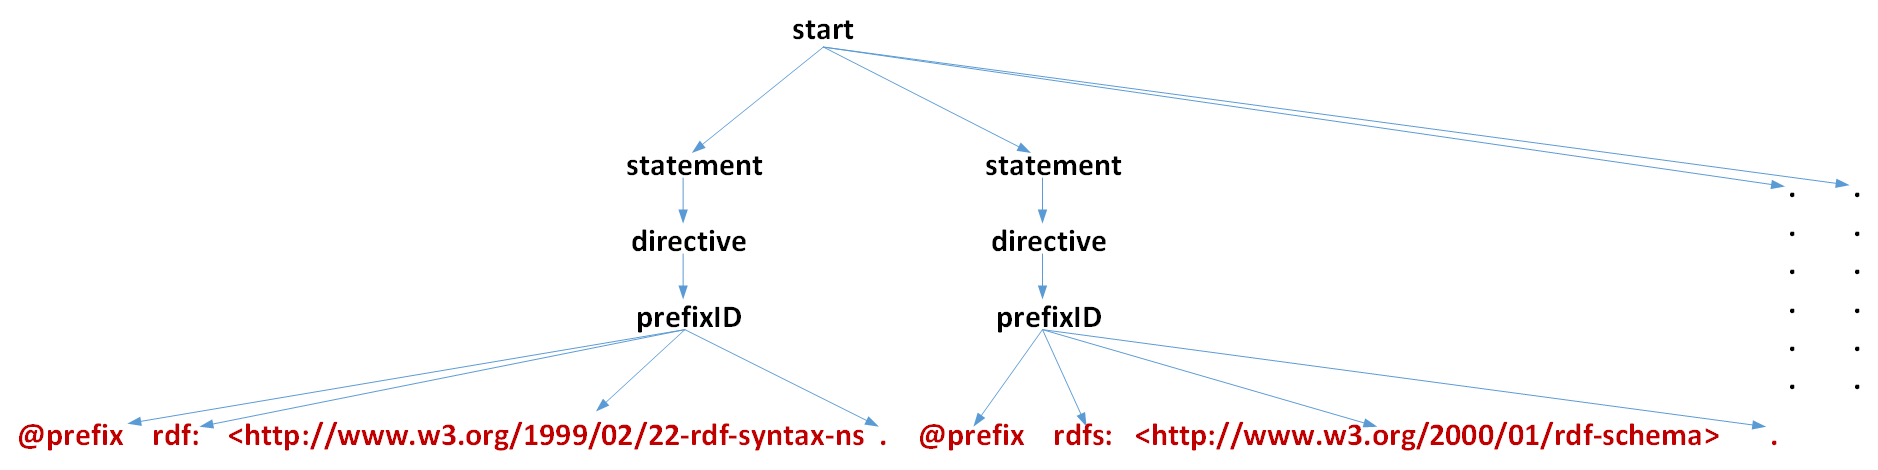
\includegraphics[width=1\linewidth]{images/implementationParseTreeLeft.png}
		\caption{\textbf{Left-side view of parse tree for Listing~\ref{lst:turtleExample}.} The view shows left-side sub-trees of the parent node start of the parse tree and it also demonstrates the hierarchy of applying grammar rules where all nodes written in \emph{black} are non-terminals or heads of the grammar rules, remaining nodes are terminals or matched patterns of input tokens.}
	\label{Fig:implementationParseTreeLeft}
\end{figure}



After showing a part of grammar rules and views of the parse tree, some of real use cases of injecting of an error production rule to match a syntax error pattern,  handling of the error detection and finally resolving the error  will be presented:

\begin{enumerate}
    \item \textbf{Missing a dot at the end of a triple:} in the Turtle syntax, a triple must end with a dot. 
    In Listing~\ref{lst:missingDotEx}, the head rule, i.e., a \textbf{statement}, can either be a directive or a triple, both ending with a dot. 
    Equally important the last line which shows that triples without a dot can also be a sub-goal of this rule. 
    This sub-goal is considered as a normal path in a parse tree, but once the parser detects it, it sends a notification to the error listener API with an error message \emph{"Missing ’.’ at the end of a triple"}.  
    \begin{figure}
		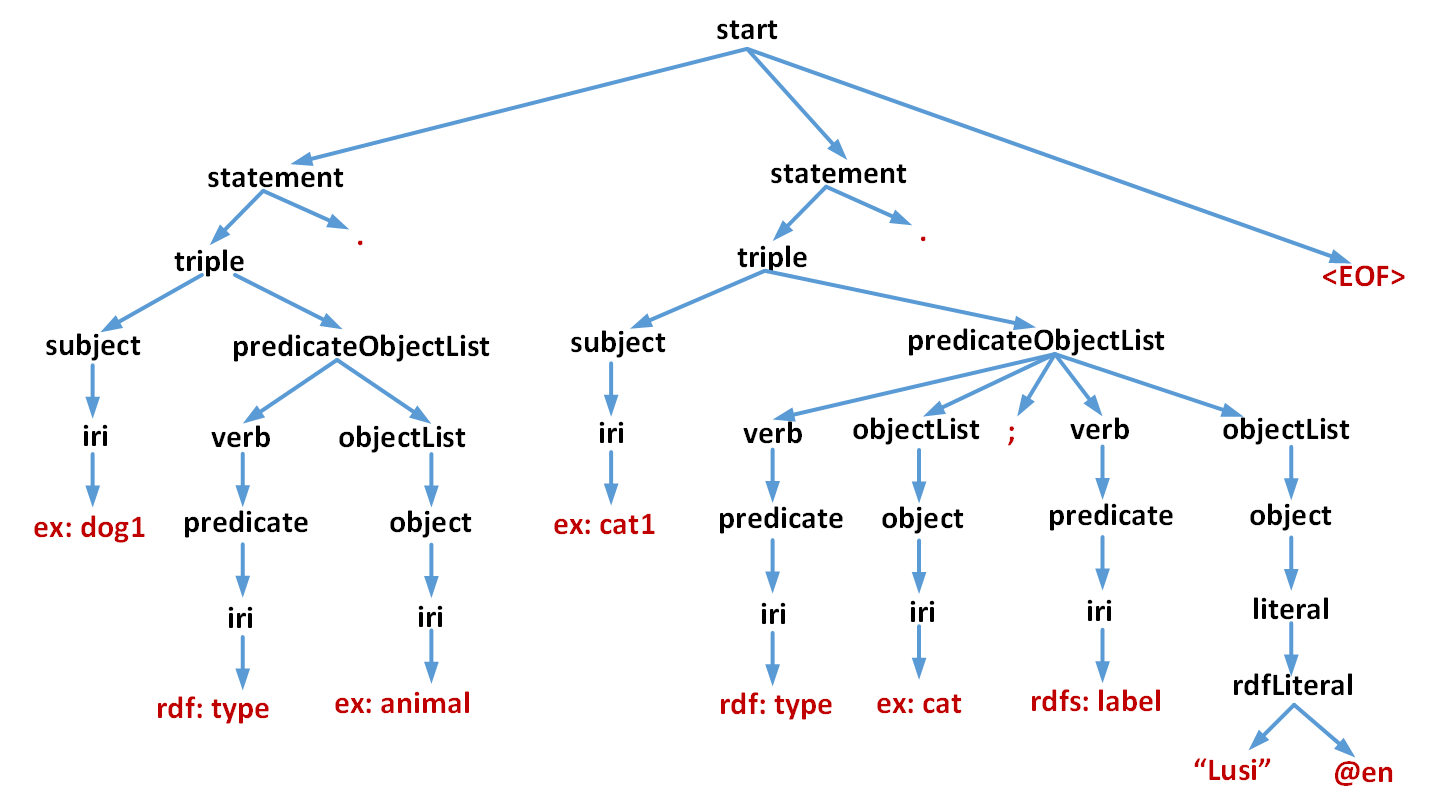
\includegraphics[width=1\linewidth]{images/implementationParseTreeRight.png}
	\caption{\textbf{Right-side view of parse tree  for listing \ref{lst:turtleExample}.} It is right-side sub-trees of the parent node \textbf{start} in the parse tree. Those nodes written in \emph{black} are non-terminals or heads of the grammar rules, remaining nodes are terminals or matched patterns of input tokens.}
	\label{Fig:implementationParseTreeRight}

\end{figure}
    
\begin{lstlisting}[label=lst:missingDotEx,  caption={Grammar rules for detecting of syntax error of missing dot at the end of a triple.}] 
statement
: directive
| triples '.'
| <@\textcolor{red}{triples  \{notifyErrorListeners("Bad end of a triple with ','")\} }@>;
\end{lstlisting}
\begin{lstlisting}[language=java, label=lst:errorCorrectionlst,  caption={Java-based handling for error recovery based on the error message in Error Correction Module.}] 
while (iterator.hasNext()) {
String line = iterator.next();
// select the action based on the error message
if (line.contains("Missing '.' at the end of Prefix
directive")||line.contains("Missing '.' at the end 
of a triple"))
<@\textcolor{violet}{addDot(lineNum, columnNum);}@>
else if (line.contains("'A' cannot be used as
predicate, it should be repalced with 'a'"))
<@\textcolor{violet}{changeA2a(lineNum, columnNum);}@>
}
\end{lstlisting}
Once such an error is saved by the Error Listener API, the role of Error Detection Module is finished. 
The next is the phase starts in the Error Correction Module to correct the error. 
Since the list of syntax error is shared with Error Correction Module, it iterates all of these errors messages, if one of these messages in the error list matches, then it applies a predefined function to recover the error.  
For instance, \textbf{addDot(lineNum, columnNum)} function is applied, as described in Listing \ref{lst:errorCorrectionlst}, since it matches the same error message and similarly, in case of \emph{"Missing  ’.’ at the end of Prefix directive"} message. 
The task of this function is to reach the line which misses the dot, identifies the line number and column number, then finally automatically corrects the error by adding a dot at the end of the given triple. 



\item \textbf{Misuse of 'A' as a predicate instead of 'a':} by mistake a user can wrongly use the character 'A' as a predicate instead of using 'a', which is the short version of the \emph{rdf:type}
If we start substitution of sub-goals of triples, \textbf{verb} can be found as a terminal node in  substitution chain. 
Syntactically, it is 'a', but if the user used 'A', then the parser will fire an error with a message of \emph{"’A’ cannot be used as a predicate, it should be replaced with ’a’"}.
Listing \ref{lst:errorCorrectionlst} also shows the handling of this error by executing \textbf{changeA2a(lineNum, columnNum)} function where the same error message is matched. 
This function can access Turtle input with the referred line number and column number, then it replaces 'A' with 'a' to correct the error. 

\begin{lstlisting}[label=lst:MissuseAex ,  caption={Grammar rules for detecting misuse of 'A' as a predicate instead of 'a'.}] 
statement
: directive
| triples '.'
;
triples
: subject predicateObjectList
;
predicateObjectList
: verb objectList (';' (verb objectList)?)*
;
verb
:'a'
| <@\textcolor{red}{'A' \{notifyErrorListeners("'A' cannot be used as predicate,         }@> 
<@\textcolor{red}{
it should be replaced with 'a'")\}} @>
;
\end{lstlisting}

\item \textbf{Bad syntax of a language tag in a literal:} 
Turtle formats has the ability to specify the language of a literal (which can be only placed as an object) by the using the character '@' followed by alphabetic characters, for example, "en", "fr", "de" are tags for English, French, German languages, respectively. 
\textbf{"Cat"@en}, and \textbf{"Katze"@de} are some examples of literals which use the language tags, the first is for English, whereas the last is for German. 


It might happen that a user instead of providing a language tag for a literal, he or she wrongly types a number, such as \textbf{"cat"@1}.
This should be considered as a syntax error in Turtle format. 
Listing~\ref{lst:badlaguageTag} handles grammar rules to make a parser firing a syntax error when such case is encountered. 

The hierarchical structure of the rules can be traversed, starting with \textbf{triples} head rule until it reaches the last two lines.
It specifies that an RDF literal can be a string followed by BAD\_LANGTAG\_AS\_NUMBER (which '@' character followed by numbers). 
When the parser finds such a pattern in the input, it delivers a syntax error to the error listener. 
Unfortunately, no error correction can be applied here, since the user intention is not easily known.  

\begin{lstlisting}[label=lst:badlaguageTag,  caption={Grammar rules for detecting incorrect language tag with a number instead of characters.}] 
triples
: subject predicateObjectList
;
predicateObjectList
: verb objectList (';' (verb objectList)?)*
;
objectList
: object (',' object)*
;
object
: literal
;
literal
: rdfLiteral
;
rdfLiteral
: String (LANGTAG | '^^' iri)?
| <@\textcolor{red}{ String  BAD\_LANGTAG\_AS\_NUMBER  \{notifyErrorListeners("Language tag cannot be a numeric value")\} }@>
;
BAD_LANGTAG_AS_NUMBER : 
'@' [0-9]+
;
\end{lstlisting}
\end{enumerate}
